%Version 3.1 December 2024
\documentclass[pdflatex,sn-mathphys-num]{sn-jnl}

\usepackage{graphicx}
\usepackage{multirow}
\usepackage{amsmath,amssymb,amsfonts}
\usepackage{amsthm}
\usepackage{mathrsfs}
\usepackage[title]{appendix}
\usepackage{xcolor}
\usepackage{textcomp}
\usepackage{manyfoot}
\usepackage{booktabs}
\usepackage{algorithm}
\usepackage{algorithmicx}
\usepackage{algpseudocode}
\usepackage{listings}

\raggedbottom

\begin{document}

\title[Melody estimation and key detection for humming]{CREPE-guided note-level melody estimation and independent key detection for monophonic humming}

\author*[1]{\fnm{Jieran} \sur{Liu}}\email{jieran\_liu@163.com}
\author[1]{\fnm{Chaoxin} \sur{Wang}}
\author[1]{\fnm{Hongyu} \sur{Jiang}}

\affil*[1]{\orgdiv{Department of Artificial Intelligence}, \orgname{Zhengzhou University of Industrial Technology}, \orgaddress{\city{Zhengzhou}, \postcode{451100}, \country{China}}}

\abstract{
Humming is a natural input modality for query-by-humming and music education systems, but converting an amateur vocal query into note-level melody remains difficult. Unlike instrumental notes, humming contains soft boundaries, pitch slides, vibrato, short unvoiced gaps and frequent intonation errors. This paper presents a compact and reproducible pipeline for monophonic humming transcription and key detection. The transcription module uses a pretrained CREPE pitch front end, frame-level acoustic descriptors and two RandomForest classifiers that separately estimate onset and offset probabilities. All transcription results are obtained with recording-grouped five-fold out-of-fold prediction on the 38 annotated recordings of the MTG-QBH/Molina corpus. The proposed system reaches a COnPOff F-measure of 0.689, improving over the strongest previously reported result on the same evaluation setting by 7.9 percentage points. Ablation experiments show that energy, spectral flux, voicing-run descriptors and temporal lag features all contribute to the final performance, while a non-learning CREPE-plus-energy baseline reaches only 0.270 COnPOff. A separate key-estimation module, based on confidence-weighted pitch-class histograms and Krumhansl-Schmuckler templates, obtains 60.5\% exact-key accuracy and 78.9\% mode accuracy against keys inferred from the ground-truth notes. We also report a negative result: forcing predicted pitches into the estimated key reduces transcription accuracy. The findings suggest that tonal information is useful as a descriptive signal for humming, but should not be used as a hard correction rule for amateur vocal pitch.
}

\keywords{humming transcription, note-level melody estimation, music information retrieval, singing voice, key detection, CREPE}

\maketitle

\section{Introduction}\label{sec:introduction}

Humming is one of the simplest ways for a non-specialist listener to describe music. It requires no instrument, no lyrics and no musical notation. This makes humming attractive for query-by-humming search, melody retrieval, singing practice tools and lightweight music-education interfaces. Behind these applications, however, lies a demanding audio analysis problem: a short and often inaccurate vocal recording has to be converted into a sequence of note onsets, offsets and pitches.

The difficulty is not only that the signal is vocal. Amateur humming differs from many instrumental transcription settings in three practical ways. First, note boundaries can be weak. A singer may connect adjacent tones with a glide, or may start a new intended note without a clear energy attack. Second, the pitch contour is continuous and expressive. Vibrato, portamento and overshoot make framewise semitone quantisation unreliable. Third, the singer may simply be out of tune. A transcription system that is too eager to enforce a global tonal model can replace the performed melody with a cleaner but less faithful one.

Earlier work on singing transcription has treated this problem through pitch tracking followed by note segmentation \cite{molina2015sipth,yang2017probabilistic,fu2019hierarchical}. More recent systems increasingly use neural sequence models, phoneme-aware representations or large singing corpora \cite{yong2023phoneme,park2023transformers,li2024rosvot,guo2025stars,kim2025timealigned}. A particularly relevant benchmark for the present study is the phoneme-informed monophonic vocal segmentation pipeline of Li et al. \cite{li2021phoneme}, which reports note-level metrics on the MTG-QBH/Molina evaluation set. Their strongest configuration reaches a COnPOff F-measure of 0.610 on the 38 recordings with note-level ground truth. That result is valuable because it uses a public corpus and a metric set designed for singing transcription, but the approach also relies on phoneme-related information that is less convenient for language-agnostic humming interfaces.

This paper revisits the same setting with a deliberately small design. We use CREPE \cite{kim2018crepe} as a pretrained fundamental-frequency front end, construct a set of frame-level pitch, energy, spectral and voicing-context features, and train two RandomForest classifiers \cite{breiman2001random}: one for note onsets and one for note offsets. The classifiers are evaluated under a strict recording-grouped out-of-fold protocol, so every recording is predicted by models that were not trained on that recording. In parallel, we add a key detector based on pitch-class template matching. The key detector is reported as an independent module rather than as a post-processing rule for note pitches. The two-branch design is summarised in Fig. \ref{fig:pipeline}.

\begin{figure}[!htbp]
\centering
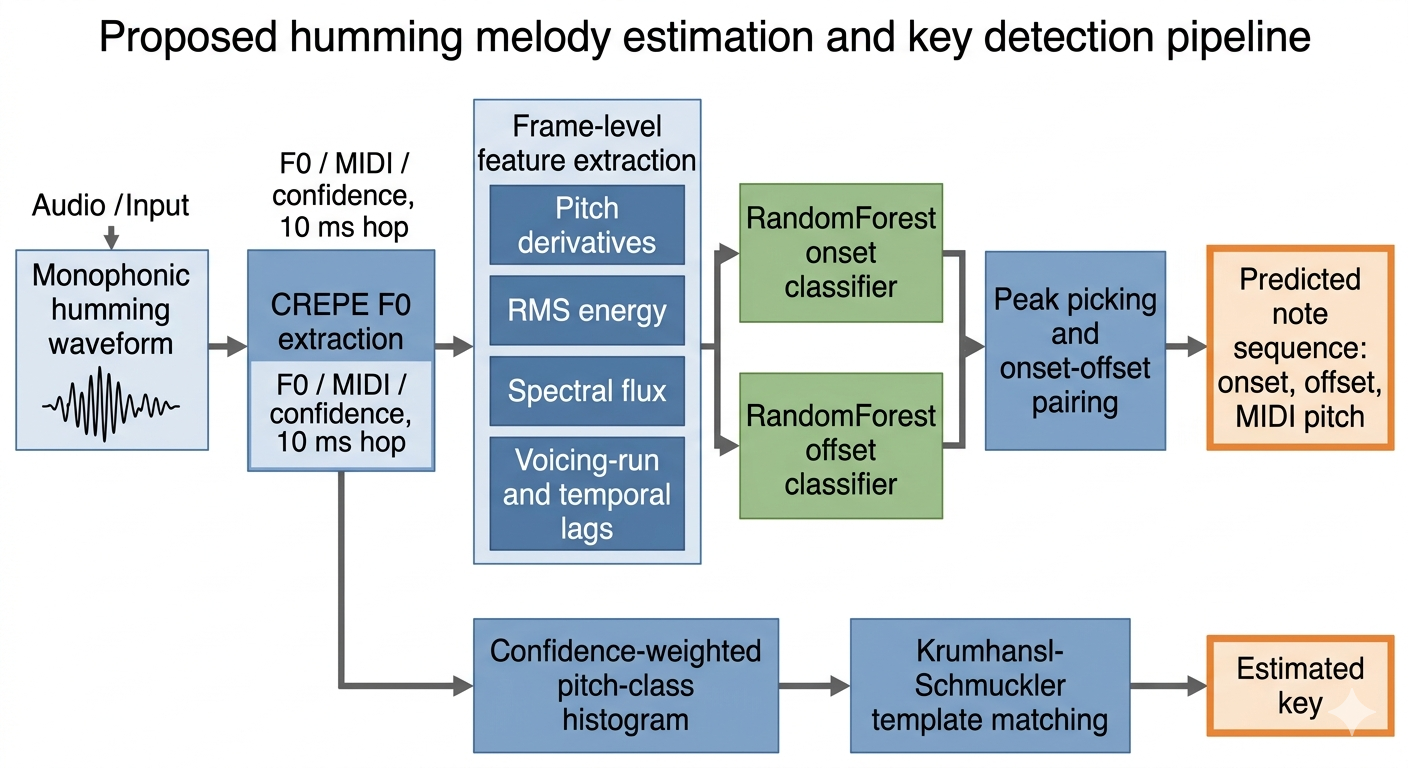
\includegraphics[width=\linewidth]{fig_pipeline.png}
\caption{Overview of the proposed humming melody estimation and key-detection pipeline. The note transcription branch uses CREPE-derived frame features and separate onset/offset RandomForest classifiers, while the key-estimation branch operates independently on the pitch-class histogram.}
\label{fig:pipeline}
\end{figure}

The main contributions are as follows.

\begin{itemize}
\item We present a reproducible note-level melody estimation pipeline for monophonic humming using CREPE-derived pitch and lightweight acoustic features.
\item On the 38 annotated MTG-QBH/Molina recordings, the proposed method reaches 0.689 COnPOff, 0.831 COnP and 0.864 COn, improving the strongest previously reported COnPOff result on this setting by 7.9 percentage points.
\item We provide ablation, non-learning baseline and bootstrap analyses that show where the gain comes from and how stable it is across recordings.
\item We evaluate an independent key-detection module and show that hard key-based pitch snapping is harmful for amateur humming, even though key estimation itself is a useful descriptive signal.
\end{itemize}

The rest of the paper is organised as follows. Section \ref{sec:related} reviews singing transcription, pitch tracking and key estimation. Section \ref{sec:data} describes the corpus and evaluation protocol. Section \ref{sec:method} gives the proposed pipeline. Section \ref{sec:experiments} reports the transcription results. Section \ref{sec:key} presents key detection. Section \ref{sec:discussion} discusses limitations and the negative key-snapping result.

\section{Related work}\label{sec:related}

\subsection{Pitch tracking and note segmentation}

Automatic music transcription has a long history in music information retrieval, but singing remains a difficult case because vocal pitch is rarely stable \cite{benetos2013amt,gomez2013flamenco}. A standard monophonic singing pipeline first estimates a frame-level pitch contour and then groups the contour into notes. Classical front ends such as YIN \cite{decheveigne2002yin} and pYIN \cite{mauch2014pyin} are widely used because they provide interpretable voicing and pitch estimates. Neural pitch trackers such as CREPE \cite{kim2018crepe} offer a different trade-off: they are pretrained, robust to a range of timbres, and often behave well on vocal signals without corpus-specific tuning. Lightweight neural transcription systems have also shown that strong pretrained or compact models can be effective when the target representation is note-based rather than frame-only \cite{bittner2022lightweight}.

The second stage, note segmentation, remains the main source of error in vocal transcription. Hysteresis on the pitch-time curve \cite{molina2015sipth}, pitch dynamic models \cite{yang2017probabilistic}, hierarchical neural classifiers \cite{fu2019hierarchical} and phoneme-informed segmentation \cite{li2021phoneme} all attempt to locate the musical boundaries that are not always visible as acoustic attacks. Recent work has pushed this direction further with phoneme-informed neural networks \cite{yong2023phoneme}, transformer models for note-level singing melody transcription \cite{park2023transformers}, and robust singing-voice transcription frameworks designed to support downstream synthesis or alignment \cite{li2024rosvot,guo2025stars,kim2025timealigned}. These systems are important evidence that linguistic and large-corpus supervision can improve singing transcription. Our setting is deliberately narrower: short monophonic humming queries, a small annotated subset and no lyrics. We therefore follow the same two-stage view but avoid language-dependent features. The hypothesis is that a modest supervised boundary detector, given robust pitch and local context, can recover much of the boundary information needed for humming.

\subsection{Evaluation of singing transcription}

Molina et al. \cite{molina2014evaluation} proposed an evaluation framework for automatic singing transcription that measures not only pitch correctness but also onset and offset agreement. The COnPOff metric is especially stringent: a predicted note must match the reference onset, pitch and offset within specified tolerances. We adopt the same family of measures through \texttt{mir\_eval} \cite{raffel2014mireval}, because these metrics are directly comparable with previous monophonic singing results and expose different types of segmentation errors.

\subsection{Key detection in symbolic and audio signals}

Template-based key detection, especially the Krumhansl-Schmuckler approach \cite{krumhansl1982tonal}, remains a useful baseline for tonal analysis. It compares a pitch-class distribution with major and minor key profiles over all possible tonics. Later work has examined profile choice, duration weighting and common key confusions \cite{temperley1999key}. In this paper, key detection is not proposed as a new tonal-analysis method. It is used as an inexpensive companion signal for humming recordings and as a test of whether global tonality should be fed back into note-level transcription.

\section{Dataset and evaluation protocol}\label{sec:data}

\subsection{Corpus}

Experiments use the MTG-QBH/Molina monophonic humming corpus. The local corpus contains 132 waveform recordings. Among them, 38 recordings have note-level ground-truth files containing onset time, offset time and MIDI pitch. These 38 recordings contain 1,959 reference notes and are used for quantitative note-level evaluation. The remaining 94 recordings do not have note-level ground truth and are used only for descriptive key-distribution analysis.

The ground-truth files do not contain manually annotated keys. For the key-detection experiment, a reference key is therefore inferred from each ground-truth note sequence by duration-weighted Krumhansl-Schmuckler matching. This reference is used only for evaluating the key-estimation module. It is not used for training the note-level boundary classifiers, selecting note pitches or scoring transcription.

\subsection{Out-of-fold evaluation}

Because only 38 recordings have note-level annotations, leakage between frames from the same recording would overstate performance. We therefore use \texttt{GroupKFold} with five folds, grouping by recording. For each fold, both the onset and offset classifiers are trained on recordings in the training split and then applied to the held-out recordings. The five held-out predictions are concatenated to form out-of-fold probability streams for all recordings. All reported transcription metrics are computed from these out-of-fold predictions.

\begin{figure}[!htbp]
\centering
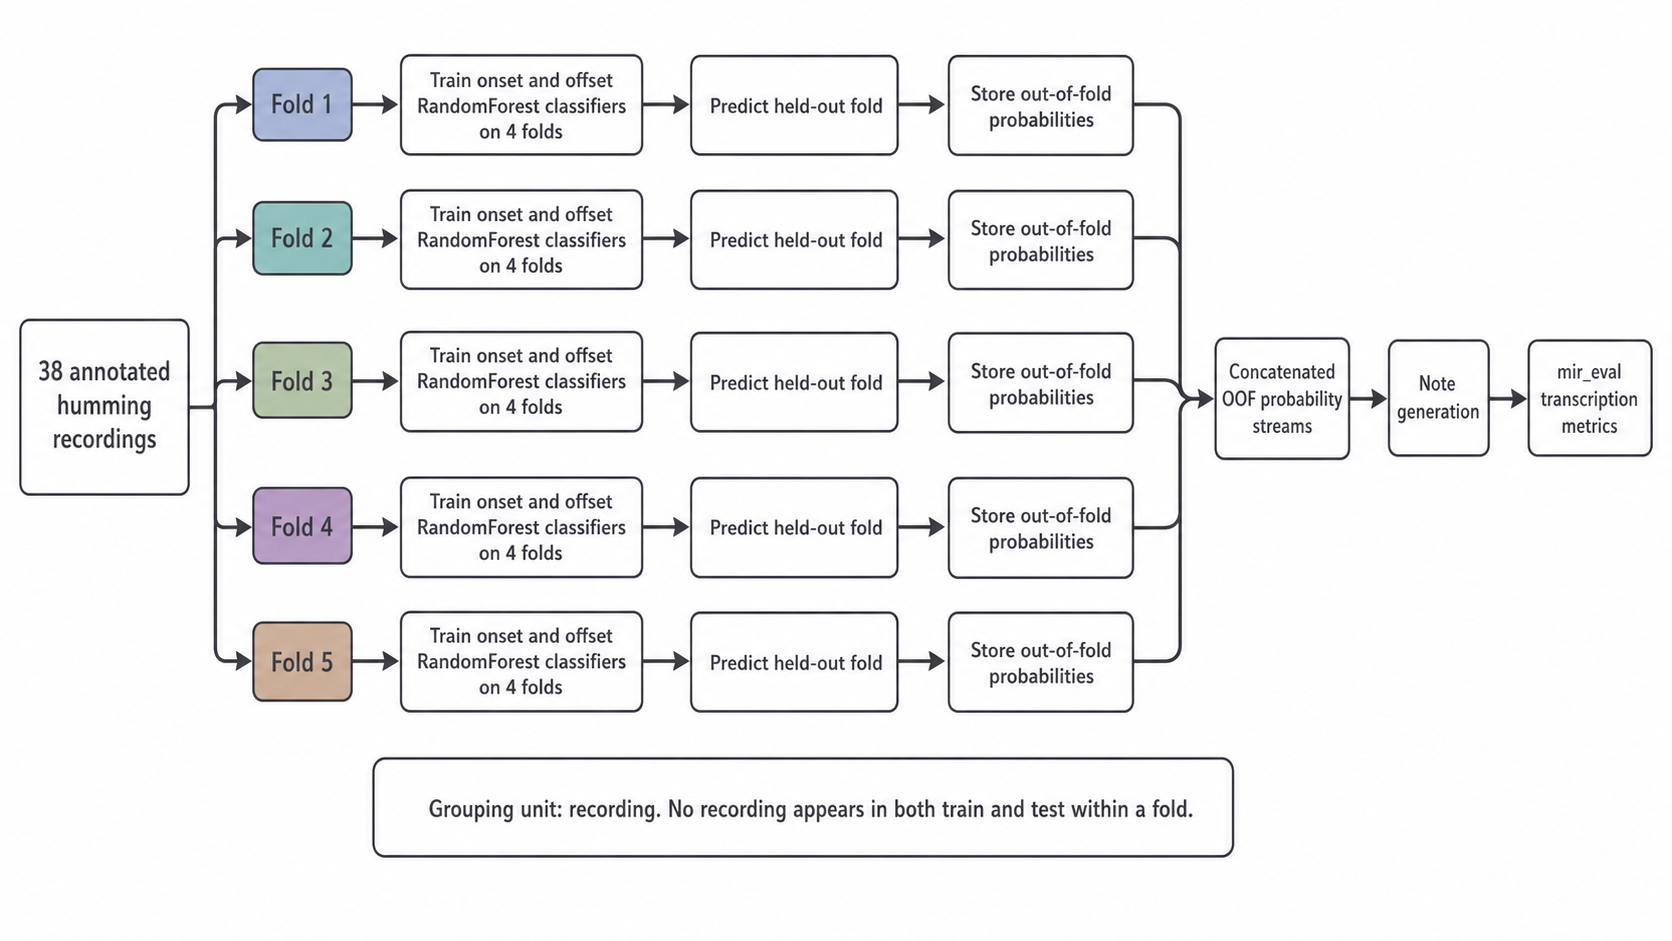
\includegraphics[width=\linewidth]{fig_oof_protocol.png}
\caption{Recording-grouped five-fold out-of-fold evaluation protocol. Each fold trains the onset and offset classifiers on four recording groups and predicts the held-out group; the five held-out probability streams are then concatenated for note generation and metric computation.}
\label{fig:oof_protocol}
\end{figure}

Figure \ref{fig:oof_protocol} summarises this evaluation design. The post-decision parameters are selected by grid search on the out-of-fold probability streams. The selected operating point is an onset probability threshold of 0.40, an offset probability threshold of 0.45, a minimum onset separation of 0.18 s and a minimum note duration of 0.10 s. This protocol should be read as recording-grouped cross-validation rather than as an independent held-out test. We return to this point in the limitations.

\subsection{Metrics}

We report the metric set used by Li et al. \cite{li2021phoneme}: COnPOff, COnP, COn, Split, Merged and Spurious. COnPOff is the F-measure for correct onset, pitch and offset. COnP ignores the offset criterion, and COn evaluates onset agreement alone. The onset tolerance is 50 ms, the pitch tolerance is 50 cents, and the offset tolerance is the maximum of 20\% of the reference duration and 50 ms. Split, Merged and Spurious describe segmentation failures following the singing-transcription evaluation tradition \cite{molina2014evaluation}. Higher is better for COnPOff, COnP and COn; lower is better for the segmentation error rates.

\section{Proposed method}\label{sec:method}

\subsection{Overview}

The proposed system follows the two-branch design introduced in Fig. \ref{fig:pipeline}. The transcription branch converts a waveform into note intervals and note pitches. CREPE first estimates a frame-level fundamental frequency and confidence. Acoustic features are then calculated at a 10 ms frame rate. Two RandomForest classifiers produce onset and offset probabilities. Peak picking and interval pairing convert the probabilities into candidate notes, and the median pitch inside each interval gives the final note pitch. The key branch uses the same pitch stream but does not influence the note predictions.

\subsection{Frame-level pitch and voicing}

CREPE is run at 16 kHz with a 10 ms hop. Each frame provides a frequency estimate, its MIDI equivalent and a confidence value. Frames below a confidence threshold of 0.25 or without valid frequency are treated as unvoiced. Very short unvoiced gaps inside voiced regions are filled by linear interpolation in the MIDI domain. This stabilises the feature stream while avoiding a hard decision about note boundaries.

\subsection{Acoustic feature set}

Each frame is represented by 44 features. The base pitch block contains smoothed MIDI pitch, CREPE confidence, a voiced flag, first and second pitch differences, absolute first difference and local pitch standard deviation. The energy block contains RMS amplitude and its first difference. The spectral block contains positive-difference spectral flux and its first difference. The voicing-run block describes time since the start of the current voiced region, time until its end and normalised position within the voiced region. Finally, temporal lag features are appended for MIDI pitch, confidence, absolute pitch difference, RMS and spectral flux at offsets of $\pm1$, $\pm3$ and $\pm5$ frames.

The feature design is intentionally conservative. It gives the classifier local evidence about pitch movement, energy change and voiced-region context without requiring lyrics, phoneme boundaries or a recurrent model.

\subsection{Boundary labels and classifiers}

For each annotated recording, a frame is labelled as an onset-positive sample if its time is within one frame of a reference onset. Offset labels are generated in the same way around reference offsets. The two label streams are kept separate. This gives two binary classification problems with strong class imbalance, because most frames are not note boundaries.

Both classifiers are \texttt{RandomForestClassifier} models implemented with scikit-learn \cite{pedregosa2011sklearn}. The final model uses 350 trees, maximum depth 16, minimum leaf size 6 and \texttt{balanced\_subsample} class weighting. Random forests were chosen for pragmatic reasons: the labelled set is small, the features are heterogeneous, and the resulting probabilities are stable enough for threshold-based note generation.

\subsection{Note generation}

Let $p_\mathrm{on}(t)$ and $p_\mathrm{off}(t)$ be the out-of-fold onset and offset probabilities. Local maxima above their thresholds are selected as boundary candidates subject to the minimum-separation rule. Candidates outside voiced regions are rejected. Each onset is then paired with a following offset that occurs before the next onset and satisfies the minimum duration constraint. For every accepted note interval, the final pitch is the median smoothed MIDI value over voiced frames in the interval, rounded to the nearest semitone and converted to frequency for evaluation.

\subsection{Independent key estimation}

The key estimator builds a confidence-weighted pitch-class histogram from the CREPE MIDI stream. The histogram is compared with cyclic shifts of the Krumhansl-Schmuckler major and minor profiles \cite{krumhansl1982tonal}. The key with the largest cosine similarity is returned. The key estimate is used only for the key-detection results in Section \ref{sec:key}; it is not used to revise note pitches in the main transcription system.

\section{Experiments}\label{sec:experiments}

\subsection{Main transcription results}

Table \ref{tab:main} compares the proposed method with the three configurations reported by Li et al. \cite{li2021phoneme} and with a non-learning heuristic baseline implemented for this study. The heuristic uses the same CREPE pitch information and RMS energy but does not train a boundary classifier.

\begin{table}[t]
\caption{Note-level transcription results on the 38 annotated MTG-QBH/Molina recordings. Higher is better for COnPOff, COnP and COn; lower is better for Split, Merged and Spurious.}
\label{tab:main}
\begin{tabular}{@{}lcccccc@{}}
\toprule
Method & COnPOff & COnP & COn & Split & Merged & Spurious \\
\midrule
Li et al. Steps 1+2 \cite{li2021phoneme} & 0.525 & 0.712 & 0.761 & 0.013 & 0.235 & 0.128 \\
Li et al. Steps 1+3 \cite{li2021phoneme} & 0.520 & 0.683 & 0.741 & 0.079 & 0.233 & 0.114 \\
Li et al. Steps 1+2+3 \cite{li2021phoneme} & 0.610 & 0.762 & 0.807 & 0.093 & 0.078 & 0.035 \\
Heuristic (CREPE + RMS) & 0.270 & 0.423 & 0.494 & 0.399 & 0.231 & 0.199 \\
Proposed method & \textbf{0.689} & \textbf{0.831} & \textbf{0.864} & 0.156 & 0.172 & 0.081 \\
\botrule
\end{tabular}
\end{table}

\begin{figure}[!htbp]
\centering
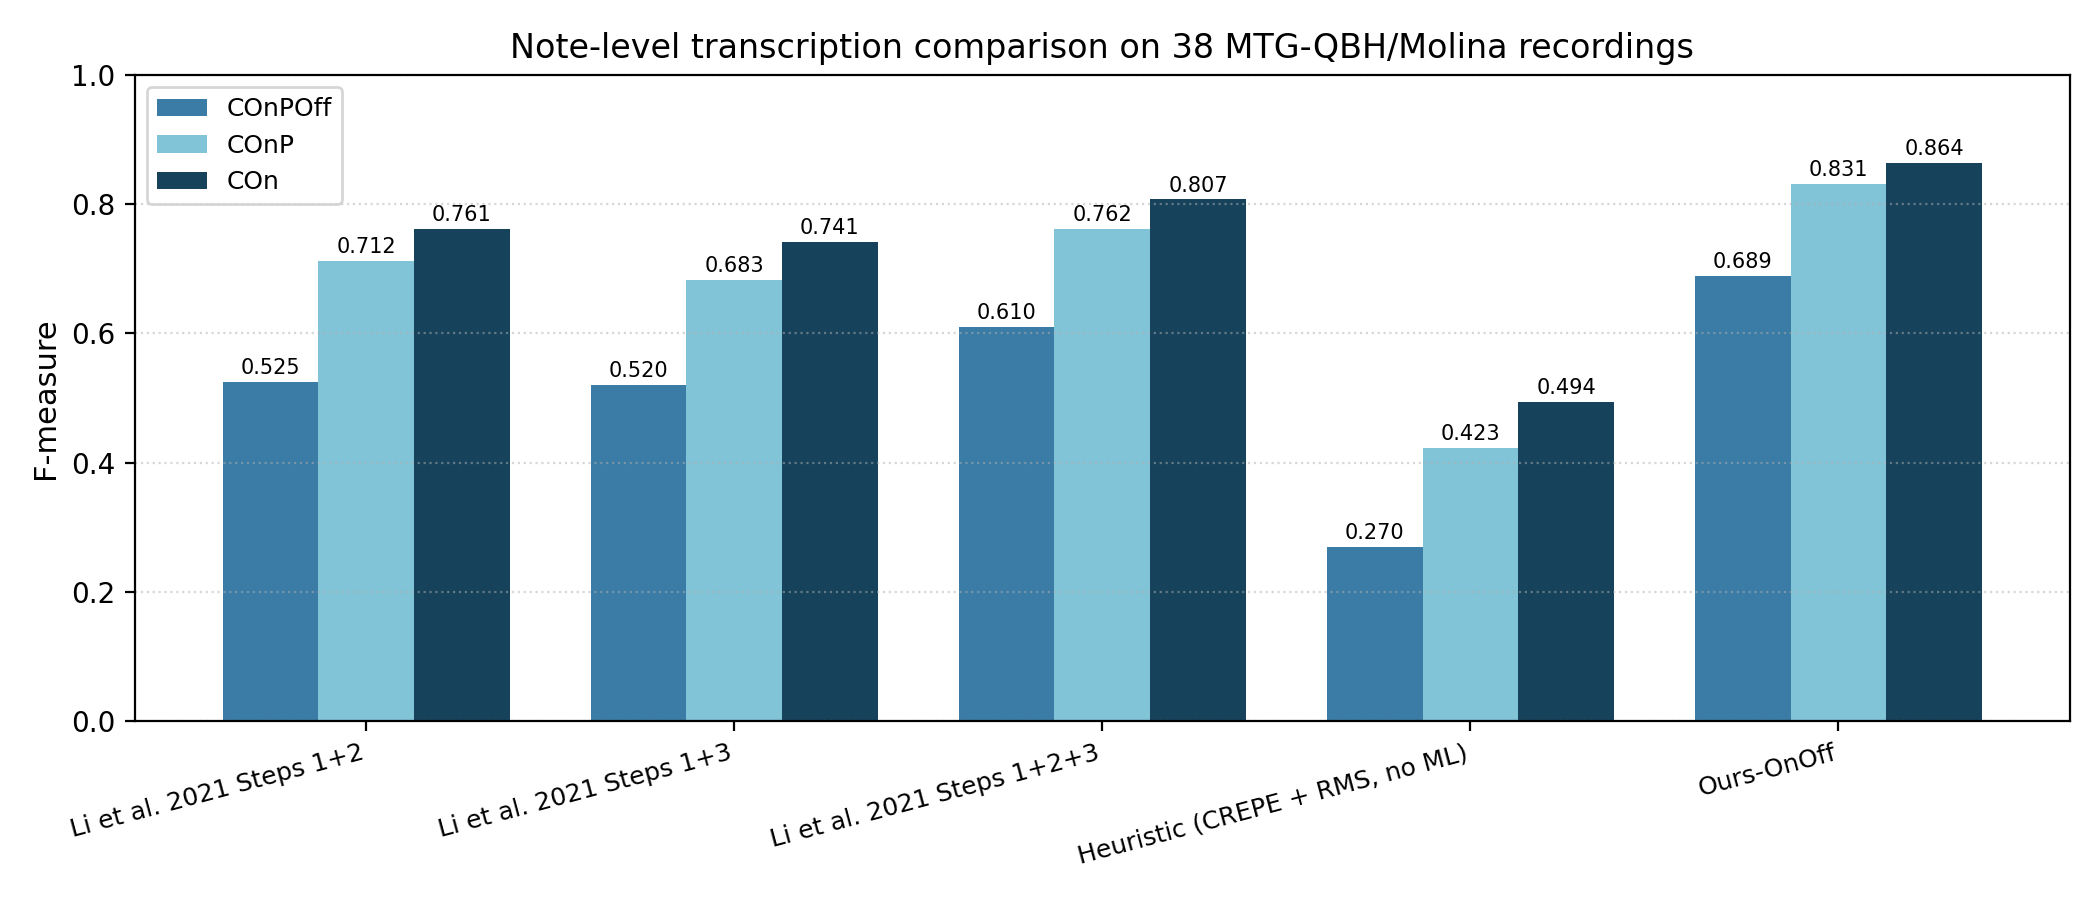
\includegraphics[width=\linewidth]{fig_method_comparison.png}
\caption{Comparison of note-level F-measures and segmentation error rates.}
\label{fig:method_comparison}
\end{figure}

The proposed method reaches 0.689 COnPOff, an absolute improvement of 7.9 percentage points over the strongest previously reported configuration in Table \ref{tab:main}. COnP and COn also improve, reaching 0.831 and 0.864. The same comparison is visualised in Fig. \ref{fig:method_comparison}, where the proposed method is consistently above the reference systems on the three F-measures. The heuristic baseline performs much worse, with 0.270 COnPOff, indicating that the supervised boundary model is responsible for most of the improvement rather than CREPE pitch tracking alone.

The segmentation error rates are more mixed. Split and Spurious are higher than in the strongest Li et al. configuration, while the note-level F-measures are higher. This is a useful trade-off to expose rather than hide. Our grid search optimises COnPOff, not segmentation purity, and the proposed system does not use phoneme-related features that may suppress some split errors. For applications where a clean symbolic score is more important than note-level matching, additional segmentation regularisation may be needed.

\subsection{Feature ablation}

Table \ref{tab:ablation} shows cumulative feature ablations. Each row adds one feature group to the previous row and retrains the same out-of-fold RandomForest pipeline. Figure \ref{fig:ablation} provides the corresponding visual comparison.

\begin{table}[t]
\caption{Cumulative feature ablation.}
\label{tab:ablation}
\begin{tabular}{@{}lcccc@{}}
\toprule
Configuration & Features & COnPOff & COnP & COn \\
\midrule
F0 only & 6 & 0.334 & 0.498 & 0.560 \\
+ RMS energy & 8 & 0.435 & 0.621 & 0.692 \\
+ spectral flux & 10 & 0.495 & 0.666 & 0.742 \\
+ voicing-run / pitch stability & 14 & 0.511 & 0.673 & 0.746 \\
+ temporal lags (full) & 44 & \textbf{0.649} & \textbf{0.778} & \textbf{0.861} \\
\botrule
\end{tabular}
\end{table}

\begin{figure}[!htbp]
\centering
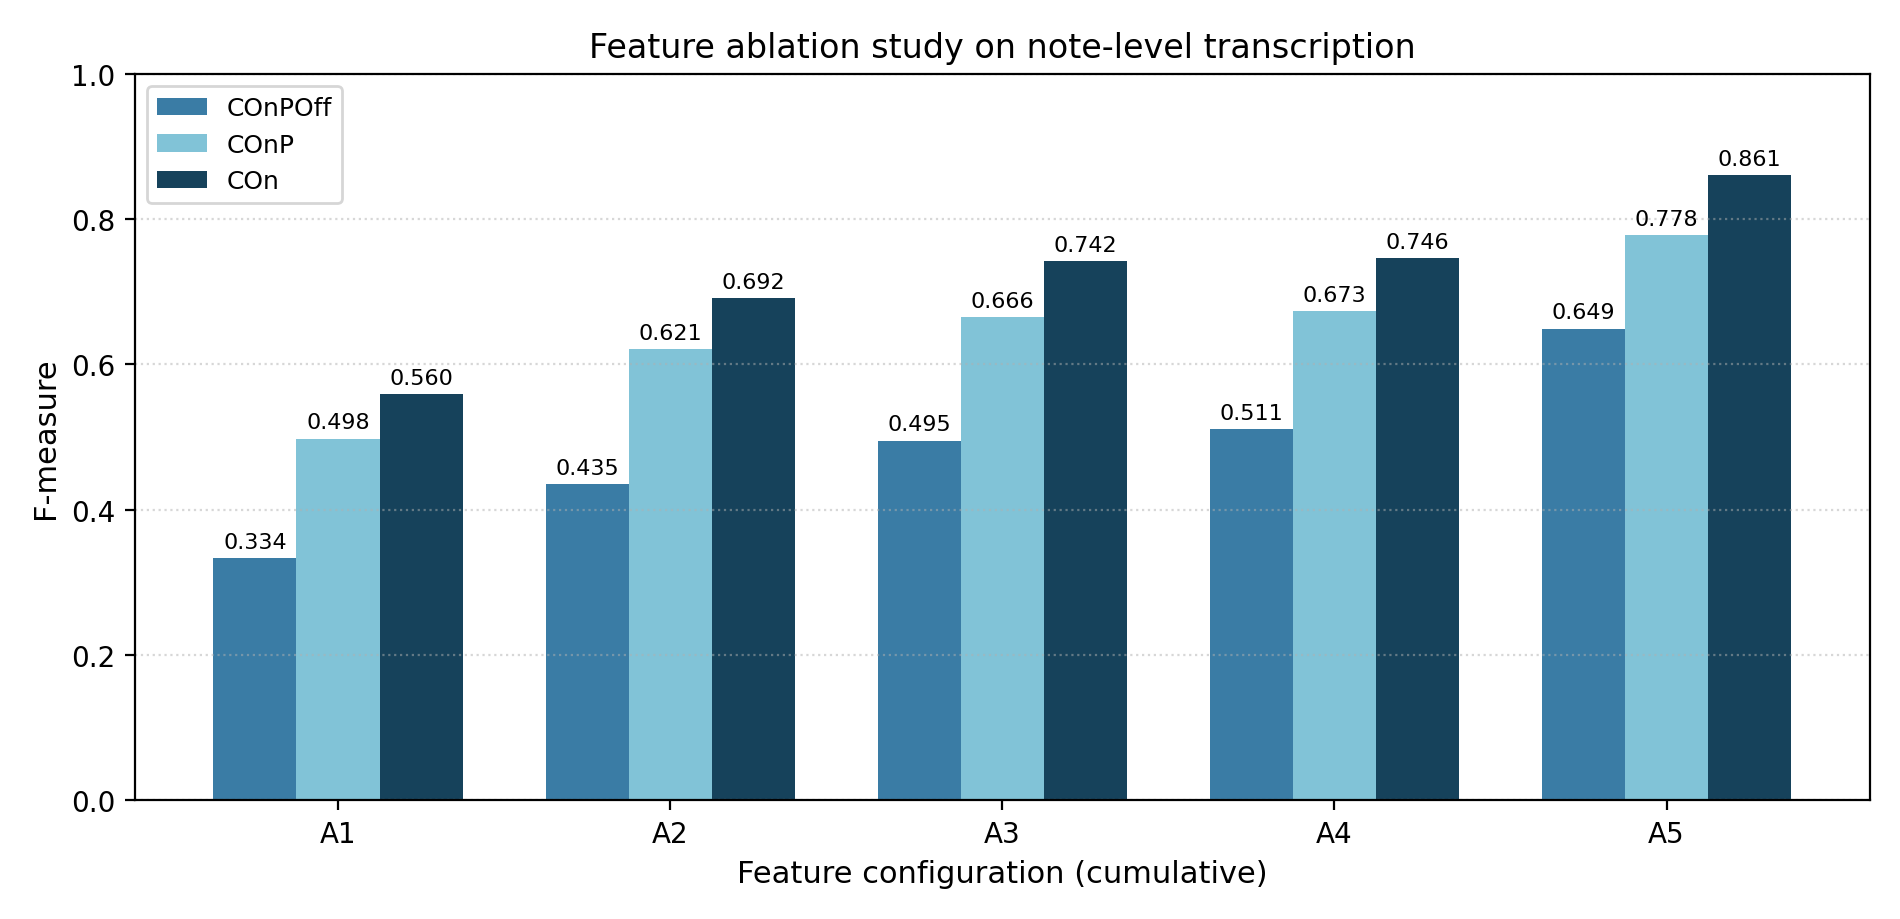
\includegraphics[width=\linewidth]{fig_ablation.png}
\caption{Feature ablation results. Temporal context produces the largest final gain.}
\label{fig:ablation}
\end{figure}

All additions improve the three F-measures. RMS energy contributes a large early gain, spectral flux adds boundary evidence beyond energy, and voicing-run features provide a small but consistent benefit. The largest single jump in Fig. \ref{fig:ablation} comes from temporal lags, which add about 14 percentage points of COnPOff over the previous configuration. This supports a simple interpretation: note boundaries in humming are often not visible in a single frame, but become clear when local motion before and after the candidate frame is available.

\subsection{Bootstrap stability}

The labelled subset is small, so a single corpus-level number is not enough. We therefore performed a recording-level bootstrap over the 38 per-recording F-measures. Table \ref{tab:bootstrap} reports the mean and percentile 95\% confidence interval over 5,000 bootstrap resamples, and Fig. \ref{fig:bootstrap} shows the corresponding bootstrap distributions.

\begin{table}[t]
\caption{Recording-level bootstrap statistics for the proposed method.}
\label{tab:bootstrap}
\begin{tabular}{@{}lccc@{}}
\toprule
Metric & Mean & 95\% CI low & 95\% CI high \\
\midrule
COnPOff & 0.621 & 0.539 & 0.693 \\
COnP & 0.756 & 0.665 & 0.835 \\
COn & 0.791 & 0.700 & 0.868 \\
\botrule
\end{tabular}
\end{table}

\begin{figure}[!htbp]
\centering
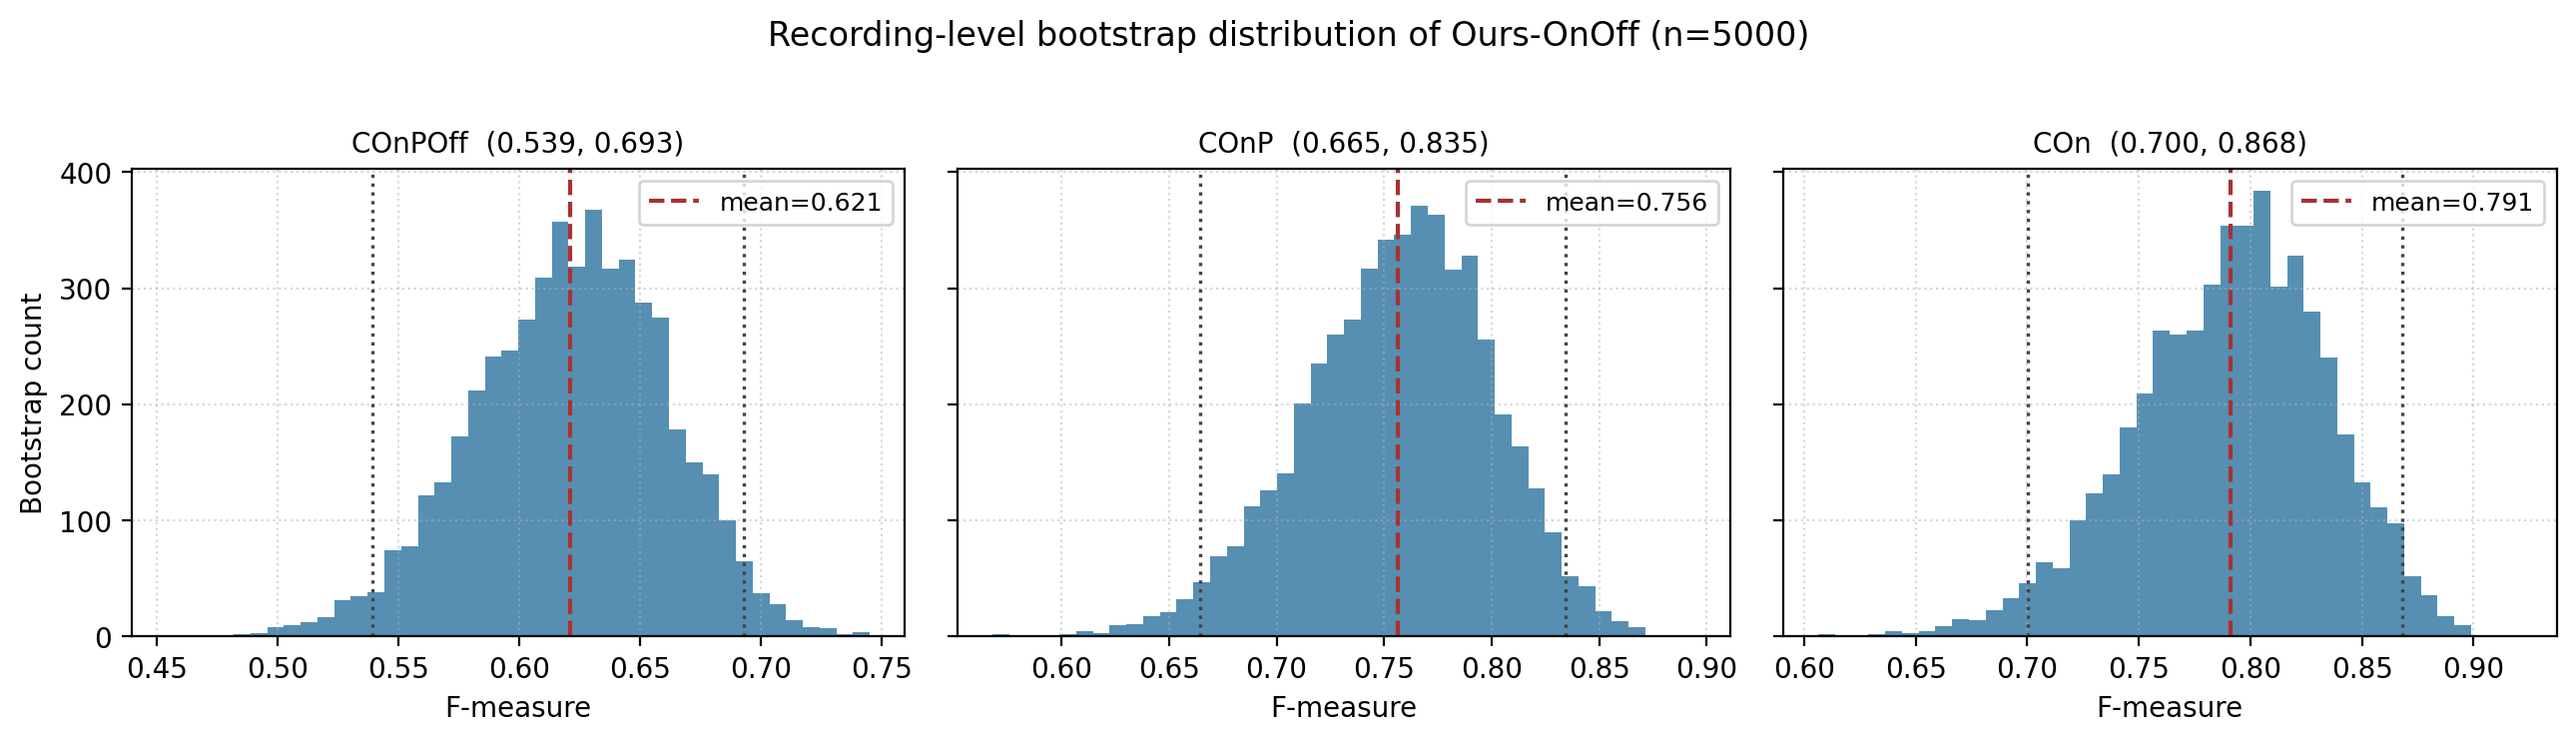
\includegraphics[width=\linewidth]{fig_bootstrap.png}
\caption{Bootstrap distributions of per-recording F-measures.}
\label{fig:bootstrap}
\end{figure}

The bootstrap mean is lower than the corpus-level COnPOff in Table \ref{tab:main} because it is a macro average over recordings, whereas Table \ref{tab:main} is computed after concatenating all recordings into a global non-overlapping timeline. The spread in Fig. \ref{fig:bootstrap} shows that the corpus contains recordings of unequal difficulty. Nevertheless, the distribution remains far above the non-learning baseline.

\subsection{Qualitative example}

Figure \ref{fig:features_child1} shows the pitch, confidence, energy and spectral-flux traces for one representative recording. Figure \ref{fig:gt_prediction_child1} overlays the predicted and reference notes. The example illustrates the behaviour seen across the corpus: many onsets are aligned tightly, while remaining errors often occur near phrase ends or weakly voiced transitions where the intended offset is perceptually ambiguous.

\begin{figure}[!htbp]
\centering
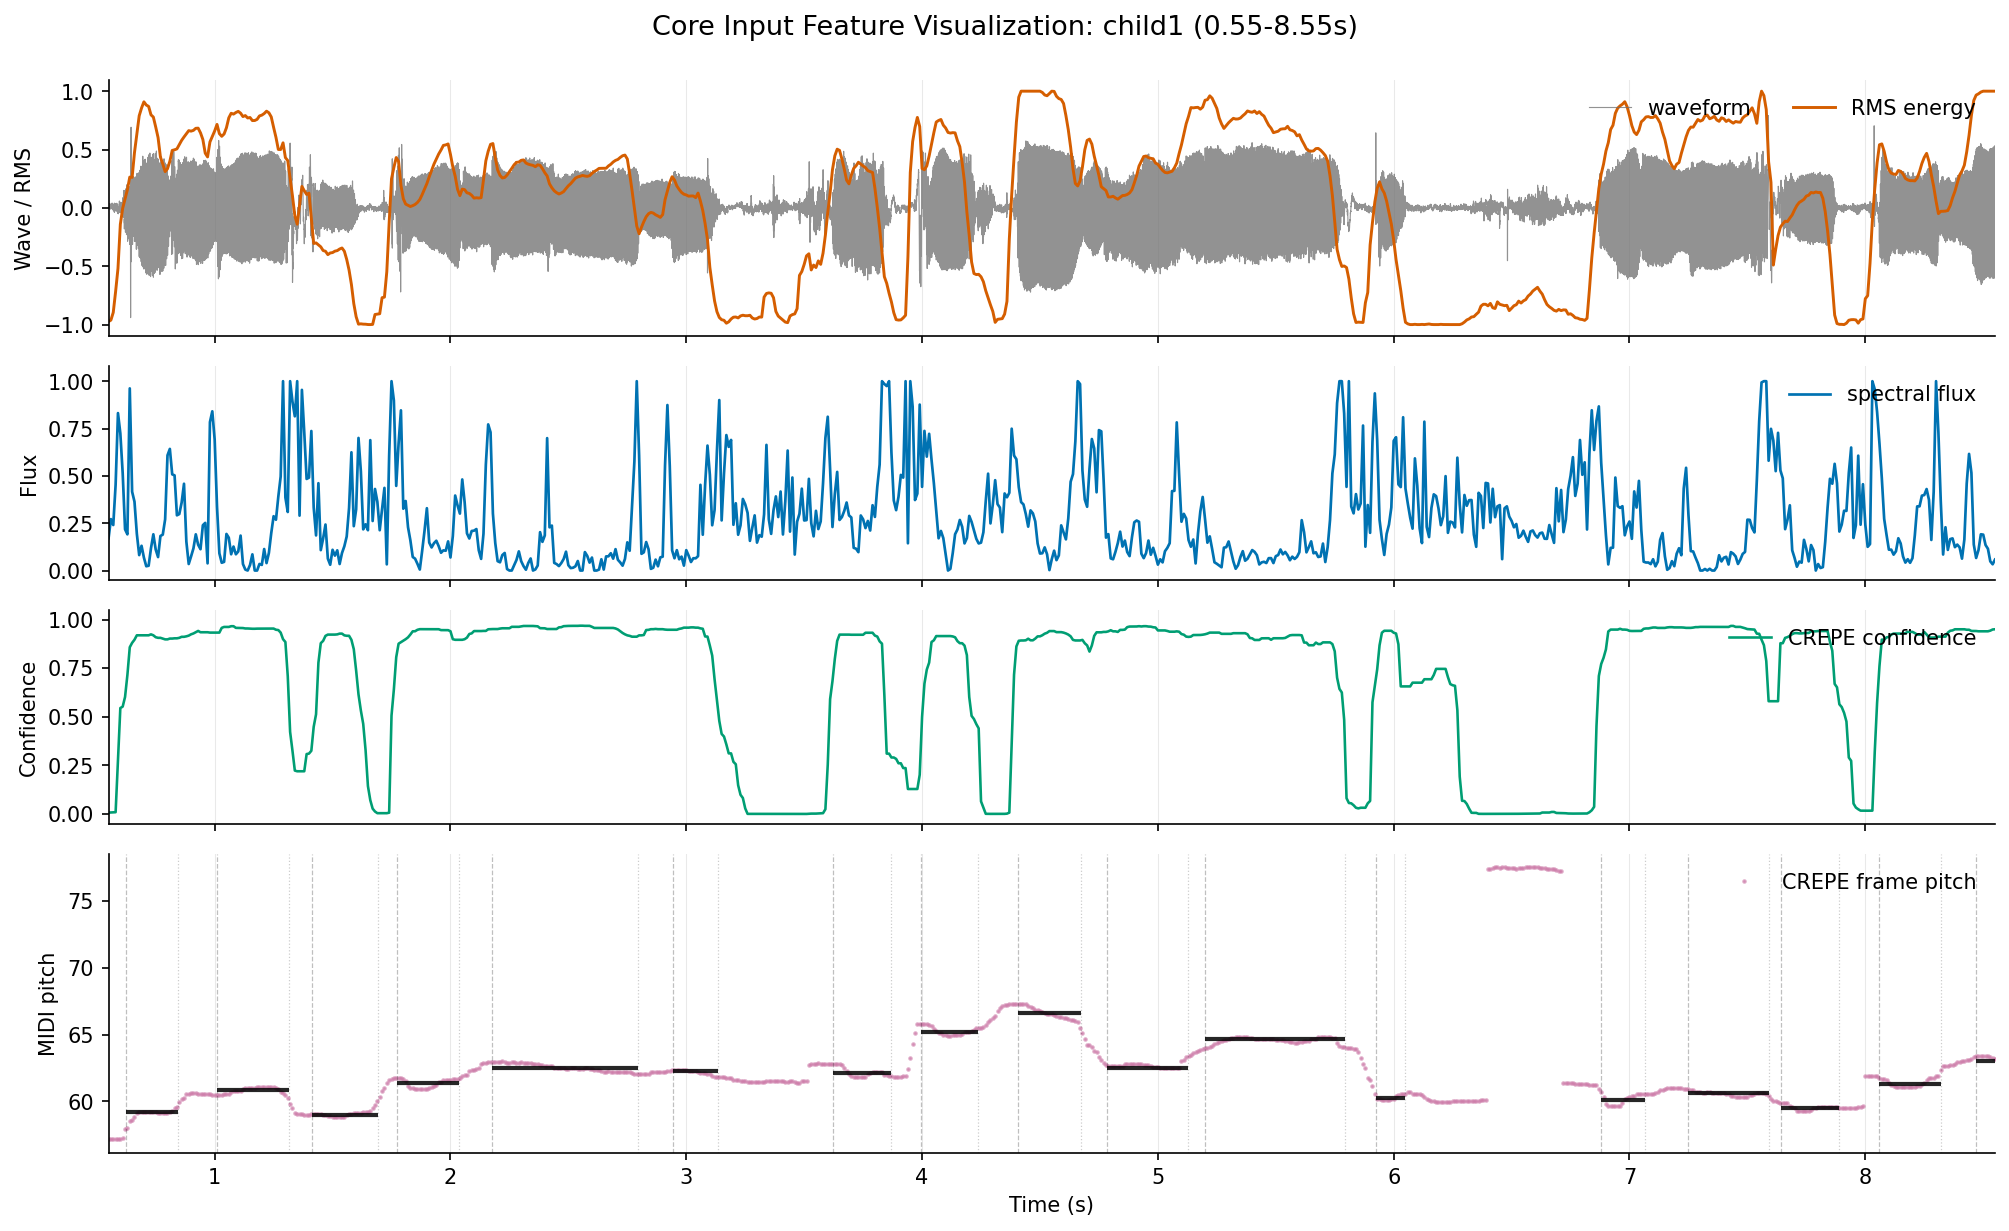
\includegraphics[width=\linewidth]{fig_features_child1.png}
\caption{Frame-level features for a representative recording.}
\label{fig:features_child1}
\end{figure}

\begin{figure}[!htbp]
\centering
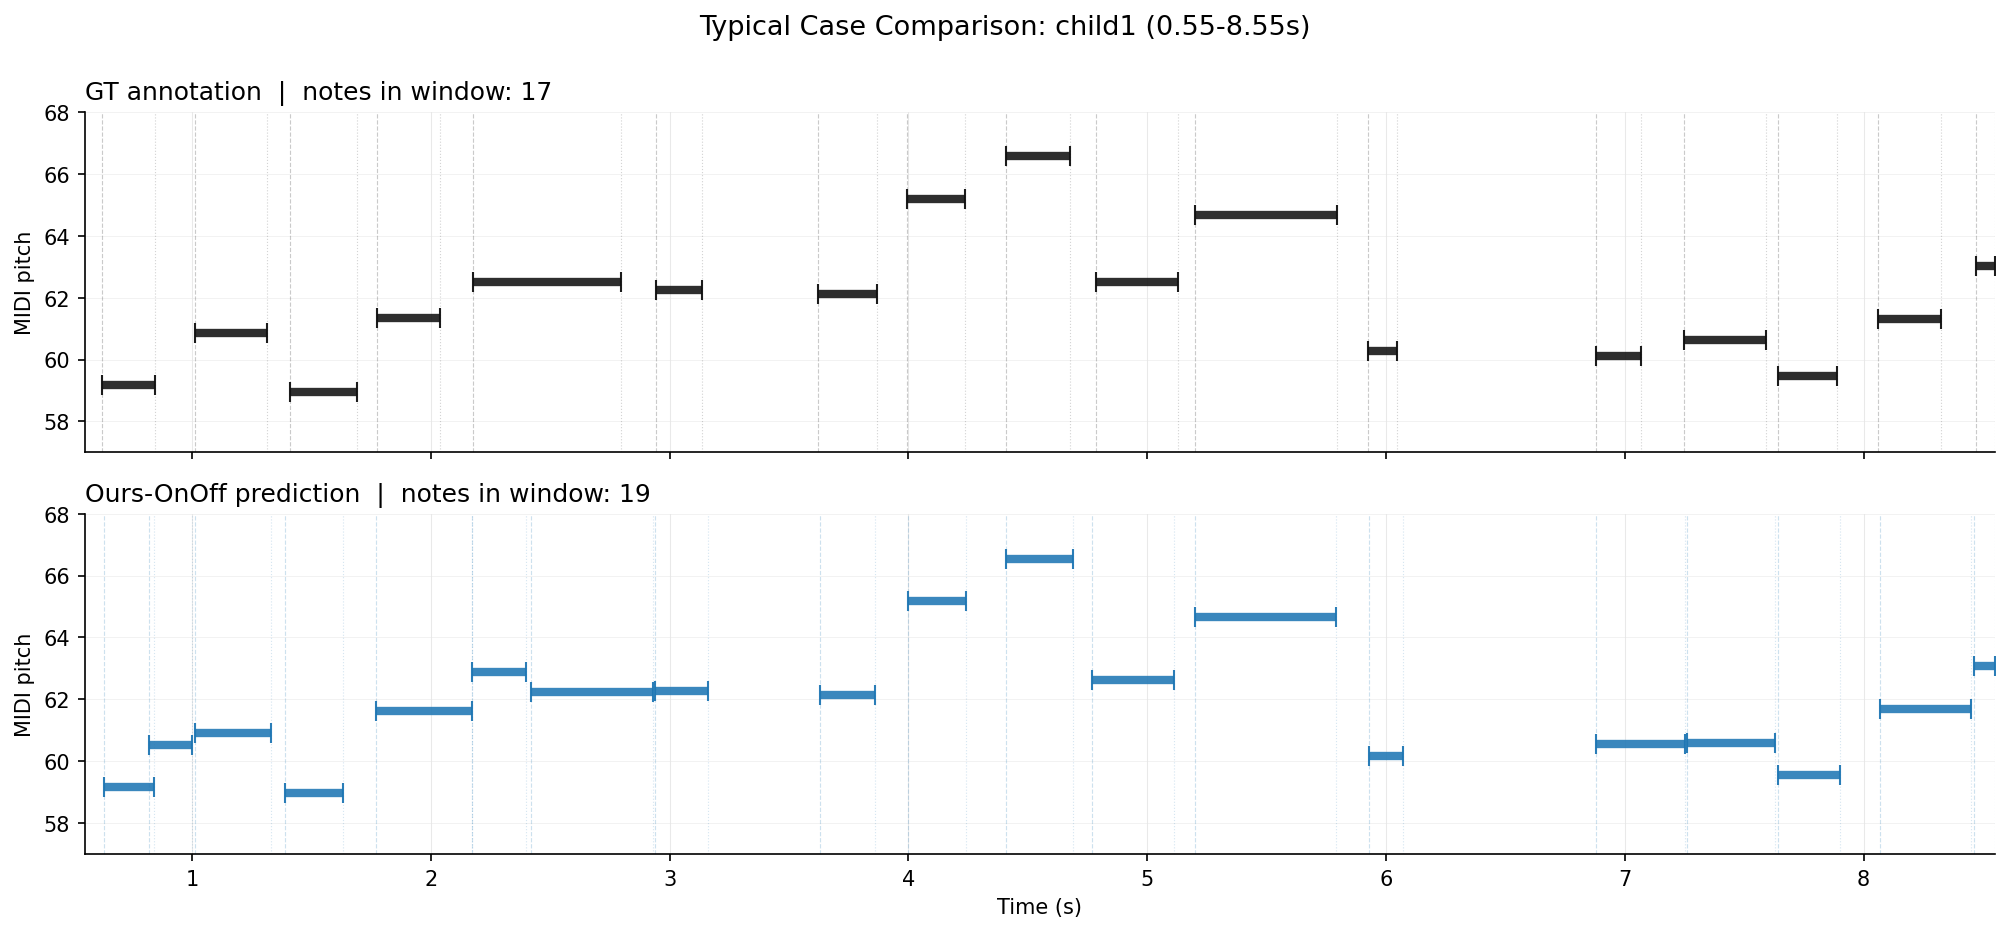
\includegraphics[width=\linewidth]{fig_gt_prediction_child1.png}
\caption{Reference and predicted notes for the same recording.}
\label{fig:gt_prediction_child1}
\end{figure}

\section{Key detection}\label{sec:key}

\subsection{Accuracy on the annotated subset}

Table \ref{tab:key} reports key-detection accuracy on the 38 recordings with ground-truth note annotations, with the same trend shown in Fig. \ref{fig:key_accuracy}. Since the corpus does not include manual key labels, the reference keys are inferred from the annotated note sequences. The strongest result is mode accuracy, where 30 of the 38 recordings are classified correctly. Exact key is more difficult, with 23 correct recordings.

\begin{table}[t]
\caption{Key-detection accuracy against keys inferred from ground-truth note sequences.}
\label{tab:key}
\begin{tabular}{@{}lcc@{}}
\toprule
Metric & Correct & Accuracy \\
\midrule
Exact key & 23/38 & 60.5\% \\
Tonic & 25/38 & 65.8\% \\
Mode & 30/38 & 78.9\% \\
\botrule
\end{tabular}
\end{table}

\begin{figure}[!htbp]
\centering
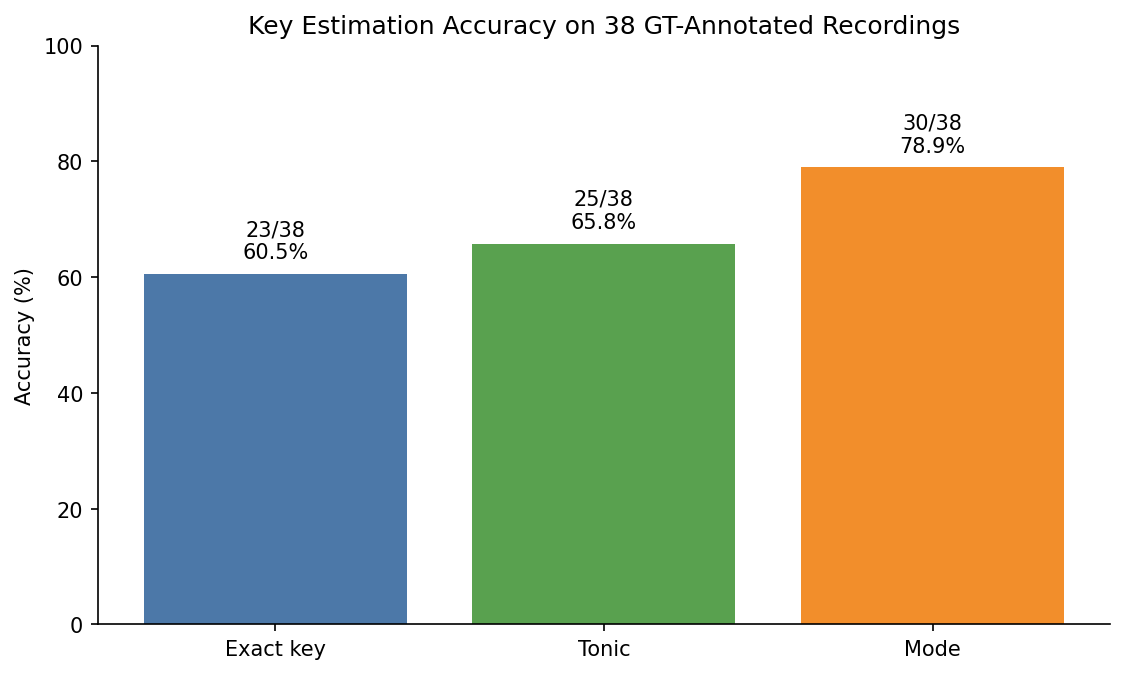
\includegraphics[width=0.75\linewidth]{fig_key_accuracy.png}
\caption{Exact-key, tonic and mode accuracy on the annotated subset.}
\label{fig:key_accuracy}
\end{figure}

These results are sufficient for corpus description and for downstream interfaces that only need a coarse tonal cue. They should not be interpreted as a claim of state-of-the-art audio key detection, because the reference keys are inferred rather than manually annotated and because the melodies are short humming queries.

\subsection{Distribution over all recordings}

The same key estimator was applied to all 132 recordings. Figure \ref{fig:mode_distribution} shows that the estimated mode distribution is almost balanced: 67 major recordings and 65 minor recordings. The tonic distribution is also spread across pitch classes, with C, C sharp, D, E flat and B among the most frequent estimated tonics. These statistics are descriptive rather than evaluative because 94 recordings do not have ground-truth note annotations.

\begin{figure}[!htbp]
\centering
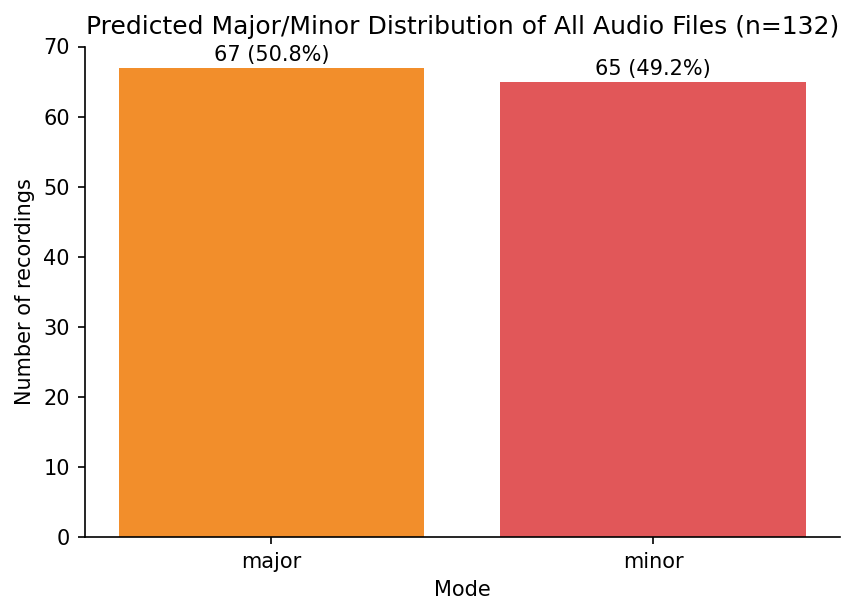
\includegraphics[width=0.68\linewidth]{fig_mode_distribution.png}
\caption{Estimated mode distribution over all 132 recordings.}
\label{fig:mode_distribution}
\end{figure}

\section{Discussion}\label{sec:discussion}

\subsection{Why a lightweight model works}

The results suggest that the hardest part of this task is not building a large model, but giving a modest model the right local evidence under a leakage-aware protocol. CREPE supplies a robust pitch contour. Energy and spectral flux supply attack and release cues. Voicing-run features tell the model whether a candidate boundary is near the beginning, middle or end of a voiced phrase. Temporal lags turn these frame descriptors into short motion patterns. With only 38 annotated recordings, this combination is better matched to the data size than a deep recurrent model trained from scratch.

\subsection{Why hard key correction fails}

A natural idea is to use the estimated key to correct the predicted note pitches. We tested this by snapping each predicted note to the nearest pitch in the estimated key. As summarised in Fig. \ref{fig:key_snapping_negative}, the result was worse: COnPOff dropped from 0.689 to 0.575. Combining this with a short-note post-processing rule degraded the result further in our exploratory experiments.

\begin{figure}[!htbp]
\centering
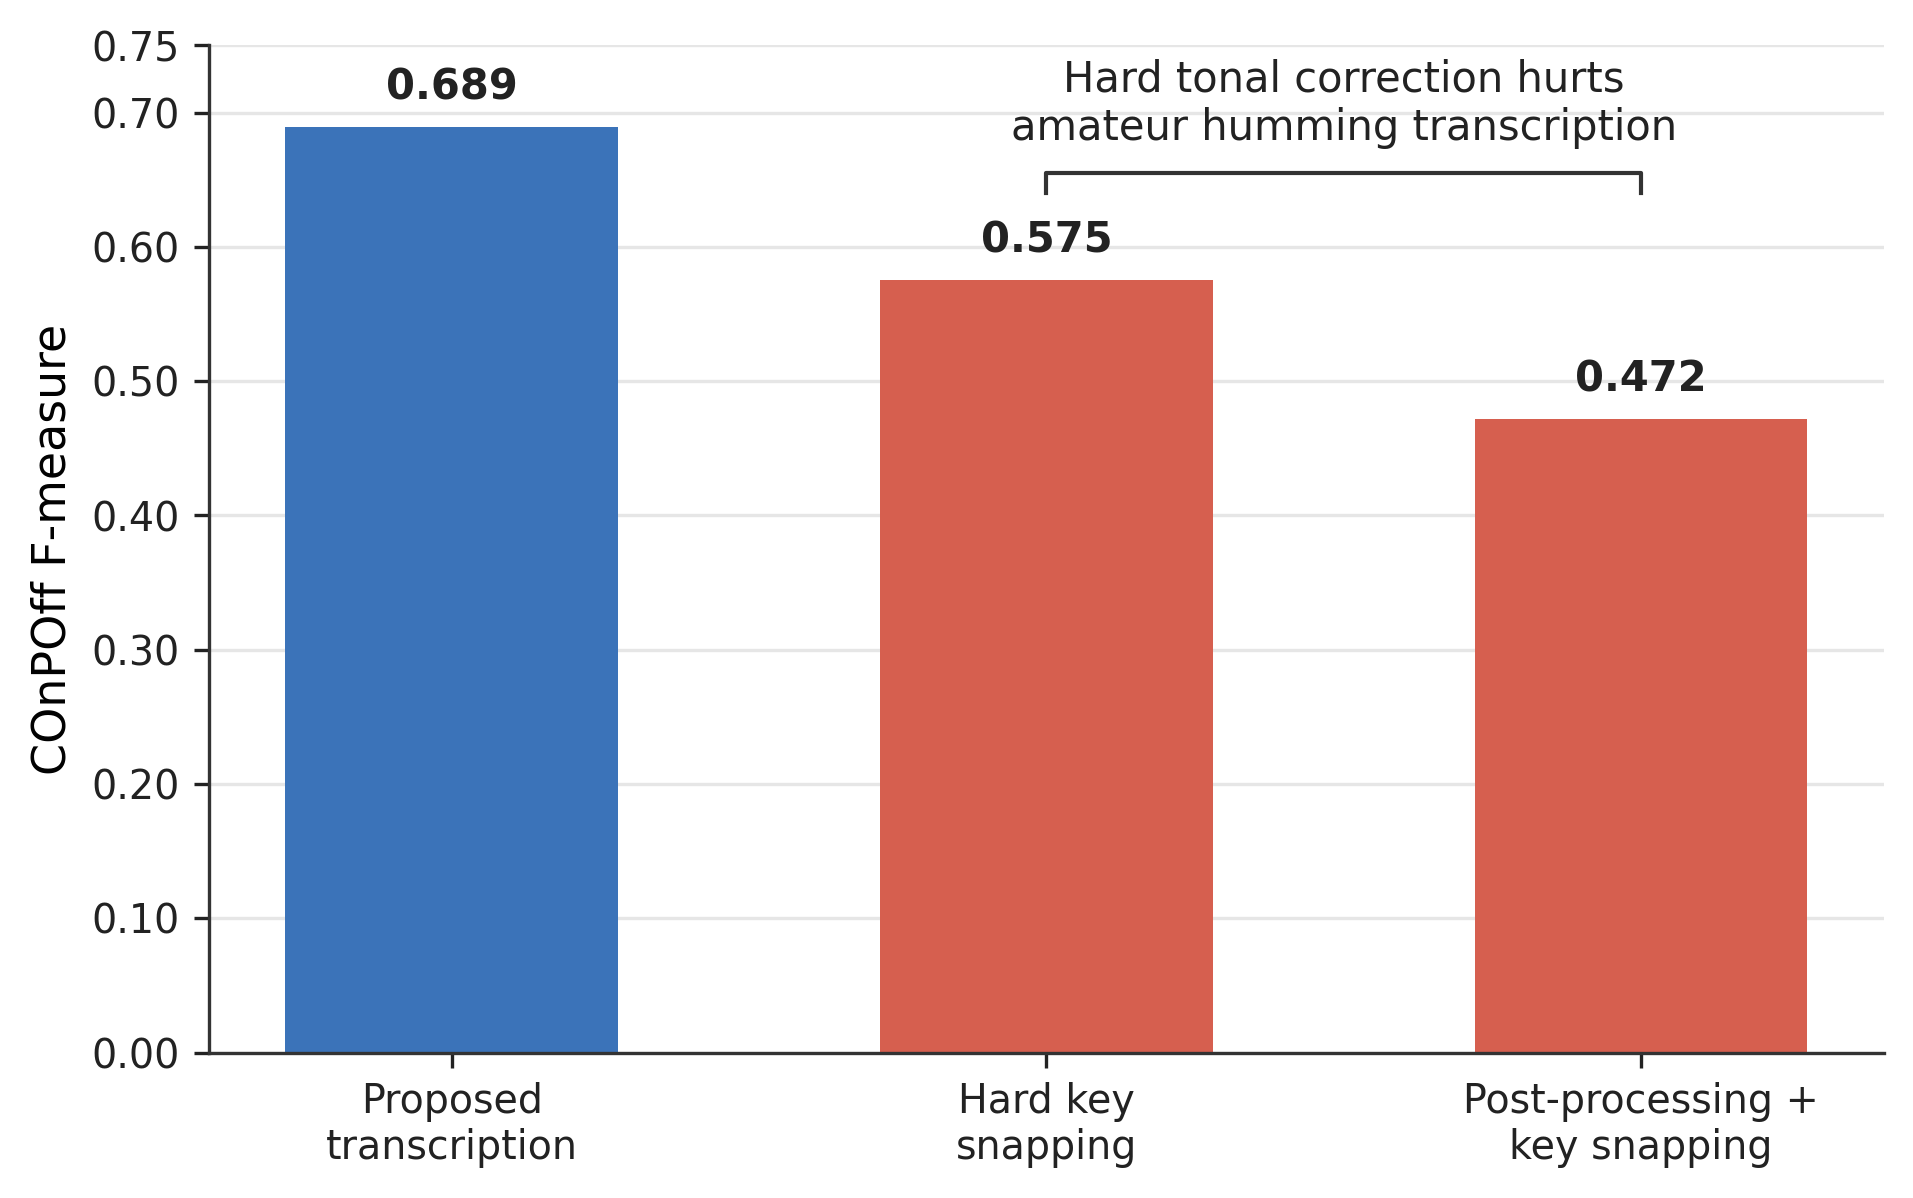
\includegraphics[width=0.72\linewidth]{fig_key_snapping_negative.png}
\caption{Negative result for hard tonal correction. Snapping predicted notes to the estimated key reduces COnPOff, and combining it with additional post-processing degrades performance further.}
\label{fig:key_snapping_negative}
\end{figure}

This failure is musically plausible. Amateur humming often contains out-of-tune but intentional contours, and a template key estimate can itself be uncertain for short queries. A hard in-key rule therefore removes information that the singer actually produced. The result supports a conservative design choice: key estimation should remain an independent signal unless the correction mechanism is soft, uncertainty-aware and trained for this specific behaviour.

\subsection{Limitations}

The main limitation is the small labelled set. Although the evaluation uses recording-grouped out-of-fold prediction, the reported operating point is still selected on the same corpus-level out-of-fold predictions. A larger held-out set or cross-corpus evaluation would provide stronger evidence. The second limitation is that the method is designed for monophonic humming; it does not address accompaniment, polyphony or lyrics-rich singing. Third, the segmentation error rates show room for improvement even when COnPOff improves. Recent phoneme-aware and sequence-model systems point to stronger boundary modelling directions \cite{yong2023phoneme,li2024rosvot,guo2025stars}, but adapting them to humming without lyrics or large aligned corpora remains an open problem. A future language-agnostic boundary cue could reduce split and spurious notes without relying on phoneme recognition.

\section{Conclusion}\label{sec:conclusion}

This paper presented a compact pipeline for note-level melody estimation and key detection in monophonic humming. Using a pretrained CREPE front end, handcrafted frame descriptors and two RandomForest boundary classifiers, the transcription module achieved 0.689 COnPOff on the 38 annotated MTG-QBH/Molina recordings under recording-grouped out-of-fold evaluation. Ablation and baseline experiments show that the gain comes from supervised boundary detection and local temporal context. The independent key detector provides useful tonal descriptors, with 78.9\% mode accuracy against ground-truth-derived reference keys, but hard key-based pitch snapping reduces transcription accuracy. For humming interfaces, the practical lesson is that tonal context should describe the query before it is allowed to correct it.

\backmatter

\bmhead{Acknowledgements}
The authors thank the creators of the MTG-QBH/Molina corpus and the authors of the open-source tools used in this study.

\section*{Declarations}

\bmhead{Funding}
No funding information has been provided at this stage. Replace this statement with the correct funding declaration before submission.

\bmhead{Competing interests}
The author declares no competing interests.

\bmhead{Ethics approval and consent to participate}
Not applicable. This study uses an existing public audio corpus and does not involve newly collected human-subject data.

\bmhead{Consent for publication}
Not applicable.

\bmhead{Data availability}
The experiments use the public MTG-QBH/Molina monophonic humming corpus. The derived frame-level features, out-of-fold probabilities, predicted note files and summary tables are prepared as supporting data for review and can be uploaded with the manuscript. A permanent public repository link should be inserted here before final submission or after acceptance, depending on the journal's review policy.

\bmhead{Code availability}
The Python scripts used to generate the reported results are available in the project repository and can be provided as supplementary material for review. A permanent repository URL should be inserted before final publication.

\bmhead{Author contributions}
J.L. designed the study, implemented the experiments, analysed the results and drafted the manuscript. C.W. and H.J. contributed to project discussion and manuscript review. All authors read and approved the final manuscript.

\bibliography{references}

\end{document}
